% *********************************************************************
% © 2026 Jeremy Sylvestre
%
% Permission is granted to copy, distribute and/or modify this document
% under the terms of the GNU Free Documentation License, Version 1.3 or
% any later version published by the Free Software Foundation; with no
% Invariant Sections, no Front-Cover Texts, and no Back-Cover Texts. A
% copy of the license is included in the appendix entitled “GNU Free
% Documentation License” that appears in the output document of this
% PreTeXt source code. All trademarks™ are the registered® marks of
% their respective owners.
%
% *********************************************************************
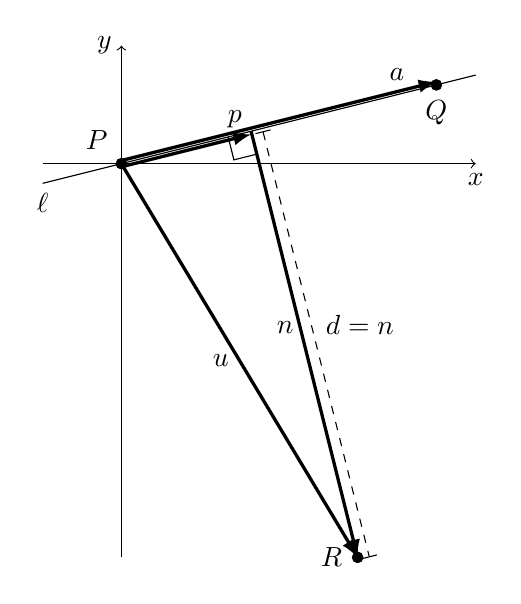
\begin{tikzpicture}[
	vector/.style={-latex,very thick},
	point/.style={circle,draw,very thin,fill,inner sep=0pt,minimum size=4pt},
	% scale=0.75
]
	% projection
	\coordinate (o) at (0,0);
	\coordinate (a) at (4,1);
	\coordinate (u) at (3,-5);
	\coordinate (p) at (1.647,0.412);

	\draw[->] (-1,0) to (4.5,0) node[below] {$x$};
	\draw[->] (0,-5) to (0,1.5) node[left] {$y$};

	% parallel to (4,1)
	\draw[thin] (-1,-0.25) to node[below,at start] {$\ell$} (4.5,1.125);

	\node[point] at (o) [label=above left:$P$] {};
	\node[point] at (a) [label=below:$Q$] {};
	\node[point] at (u) [label=left:$R$] {};

	\draw[vector] (o) to node[left] {$\uvec{u}$} (u);
	\draw[vector] ([yshift=0.04cm]o) to node[above,very near end] {$\uvec{a}$} ([yshift=0.04cm]a);
	\draw[vector] ([yshift=-0.04cm]o) to node[above,very near end] {$\uvec{p}$} ([yshift=-0.04cm]p);
	\draw[vector] (p) to node[above left] {$\uvec{n}$} (u);
	\draw[dashed,|-|] ([xshift=0.15cm]p) to node[above right] {$d = \unorm{n}$} ([xshift=0.15cm]u);

	% perp symbol
	\begin{scope}[xshift=1.647cm,yshift=0.412cm]
		\draw[thin,rotate=194.036] (0.3,0) to (0.3,0.3) to (0,0.3);
	\end{scope}

\end{tikzpicture}
